% Figure: the admissible cone, module B. Referenced from section 3 after prop:choquet-cone.
% Pure TikZ. Redrawn 2026-09-19 at the external presentation review (item 13): the first
% version placed the stable, Matern and Student-t families and the image of the bridge on rays
% inside the wedge while its caption said that "nothing is placed by the drawing". The figure
% now shows one thing, the superposition of prop:choquet-cone: a member as a Gaussian term plus
% a weighted sum of Cin rays. Class membership is Figure 4's job (the dimension filtration) and
% the inclusion chain of section 5.3.

\begin{figure}[t]
\centering
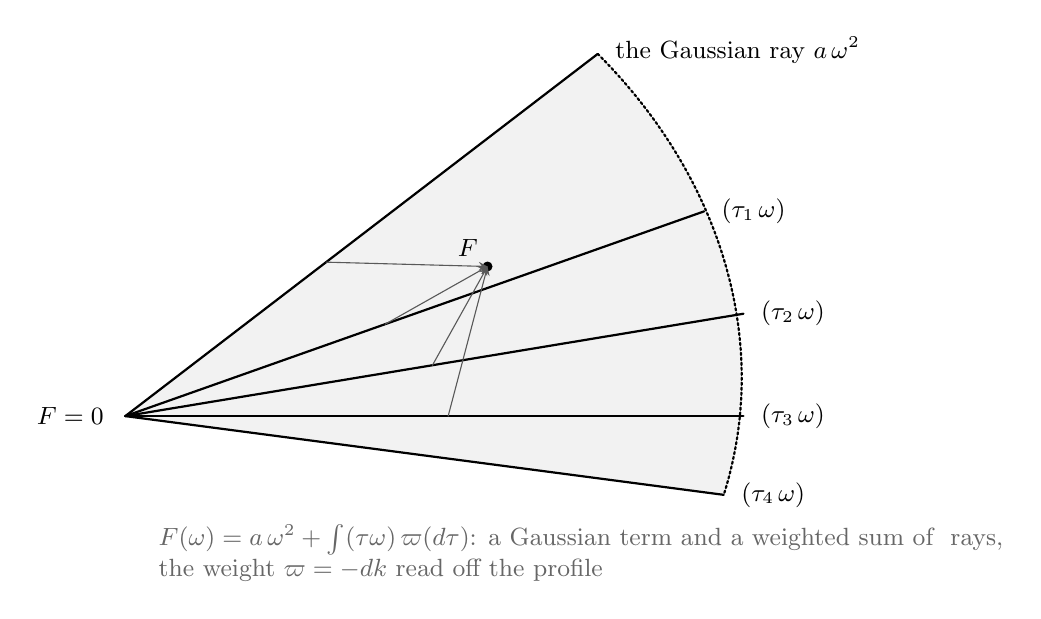
\begin{tikzpicture}[every node/.style={font=\small}, line cap=round, >=stealth]
\coordinate (O) at (0,0);
% the wedge
\fill[gray!10] (O) -- (6.0,4.6) .. controls (7.6,3.0) and (8.2,0.9) .. (7.6,-1.0) -- cycle;
\draw[thick] (O) -- (6.0,4.6);
\node[anchor=west] at (6.1,4.65) {the Gaussian ray $a\,\omega^2$};
% the Cin rays, one for each tau, along the far side
\foreach \x/\y/\lab in {7.35/2.6/{\tau_1}, 7.85/1.3/{\tau_2}, 7.85/0.0/{\tau_3}, 7.6/-1.0/{\tau_4}} {
  \draw[thick] (O) -- (\x,\y);
  \node[anchor=west] at (\x+0.1,\y) {$\Cin(\lab\,\omega)$};
}
\draw[thick, densely dotted] (6.0,4.6) .. controls (7.6,3.0) and (8.2,0.9) .. (7.6,-1.0);
\node[anchor=east] at (-0.15,0) {$F = 0$};
% a member as a superposition
\coordinate (F) at (4.6,1.9);
\fill (F) circle (1.8pt);
\node[anchor=south east] at (F) {$F$};
\draw[->, gray!70!black] (2.55,1.955) -- (F);
\draw[->, gray!70!black] (3.3,1.167) -- (F);
\draw[->, gray!70!black] (3.9,0.645) -- (F);
\draw[->, gray!70!black] (4.1,0.0) -- (F);
\node[anchor=north west, align=left, text=gray!80!black] at (0.3,-1.25)
  {$F(\omega) = a\,\omega^2 + \int \Cin(\tau\omega)\,\varpi(d\tau)$:
   a Gaussian term and a weighted sum of $\Cin$ rays,\\ the weight $\varpi = -dk$ read off the profile};
\end{tikzpicture}
\caption{The admissible cone, schematically. The exponents $F$ are the pairs $(a,k)$, a
Gaussian coefficient and a nonincreasing profile, and they form a convex cone
(Lemma~\ref{lem:admissible-cone}). Its extreme rays are the Gaussian ray, the member with no
jumps, and the $\Cin$ rays, one for each cutoff $\tau$, the exponents of the unit-step
profiles. Every member is a superposition of them in exactly one way, with the weights given
by the profile: a nonincreasing profile is a stack of unit steps, and $\varpi = -dk$ says how
much of each (Proposition~\ref{prop:choquet-cone}). The drawing shows that superposition and
nothing else; the cone has infinitely many dimensions, and where the named families and the
image of the bridge lie in it is the subject of Figure~\ref{fig:filtration} and of the chain
in \S\ref{sec:thorin}.}
\label{fig:admissible-cone}
\end{figure}
